\documentclass[a4paper,11pt,final]{article}

\usepackage[english,francais]{babel}
\usepackage[utf8]{inputenc}
\usepackage[T1]{fontenc}
\usepackage[pdftex]{graphicx}
\usepackage{setspace}
\usepackage{hyperref}
\usepackage[french]{varioref}
\usepackage{graphicx}
\usepackage[absolute]{textpos}

\newcommand{\reporttitle}{Inversion de couleurs} 
\newcommand{\reportauthor}{Valentin \textsc{Durand}} 
\newcommand{\reportsubject}{TPE : Fondements de l'informatique} 
\newcommand{\HRule}{\rule{\linewidth}{0.5mm}}
\setlength{\parskip}{1ex} 
\setlength{\textwidth}{150mm}
\setlength{\oddsidemargin}{5mm}
\setlength{\topmargin}{0mm}
\setlength{\textheight}{220mm}

\hypersetup{
    pdftitle={\reporttitle},%
    pdfauthor={\reportauthor},%
    pdfsubject={\reportsubject}
}

%% Le titre du papier
\title{TPE : \textsc{Fondements de l'informatique \\ Inversion de couleurs}}
\author{Valentin Durand, ENSICAEN -- 1A Informatique (2015-2016)}

\begin{document}

\begin{textblock*}{3cm}(85mm,20mm) 
	
\includegraphics[scale=0.2]{./pic/logo-ensicaen-2015.jpg} 
\end{textblock*} 

\maketitle

\tableofcontents
\sloppy 
\cleardoublepage

\section*{Introduction}
\addcontentsline{toc}{section}{Introduction}

Ce projet a permis de mettre en pratique les connaissances acquises en programmation C au cours du premier semestre, notamment les structures de données et les allocations dynamiques, afin de produire un programme limitant les couleurs d'une image à celles disponibles dans une table prédéfinie. Ce programme prend en paramètre une image et une table de couleur, puis se charge pour chaque pixel de chercher sa couleur la plus proche dans la table de couleur, de remplacer ce pixel par la couleur trouvée et de sauvegarder l’image finale. L’algorithme de recherche de la couleur la plus proche est décliné en deux versions, une méthode triviale assez lente et une méthode utilisant des kd arbres afin d’accélérer la durée d’exécution. Ce rapport a donc pour but de détailler l’implémentation de ces deux méthodes et de comparer leurs résultats.

\section{Méthode de travail}

Bien que ce projet ait été réalisé en monôme, un gestionnaire de version a été utilisé afin de structurer le travail à effectuer au cours des mois de décembre et janvier. Les jalons ont suivis linéairement les consignes stipulées dans l’énoncé:
\begin{itemize}
\item Familiarisation avec le module image \emph{(16 Dec)} ;
\item Création du module table de couleur \emph{(16 - 22 Dec)} ;
\item Implémentation de la méthode triviale \emph{(22 Dec - 1 Jan)} ;
\item Construction du kd arbre \emph{(1 - 2 Jan)} ;
\item Calcul de la couleur la plus proche dans l’arbre \emph{(2 Jan)} ;
\item Inversion de couleur par kd arbre \emph{(2 Jan)} ;
\item Comparaison des résultats \emph{(31 Jan)}.
\end{itemize}

\begin{figure}[ht!]
	\centering
	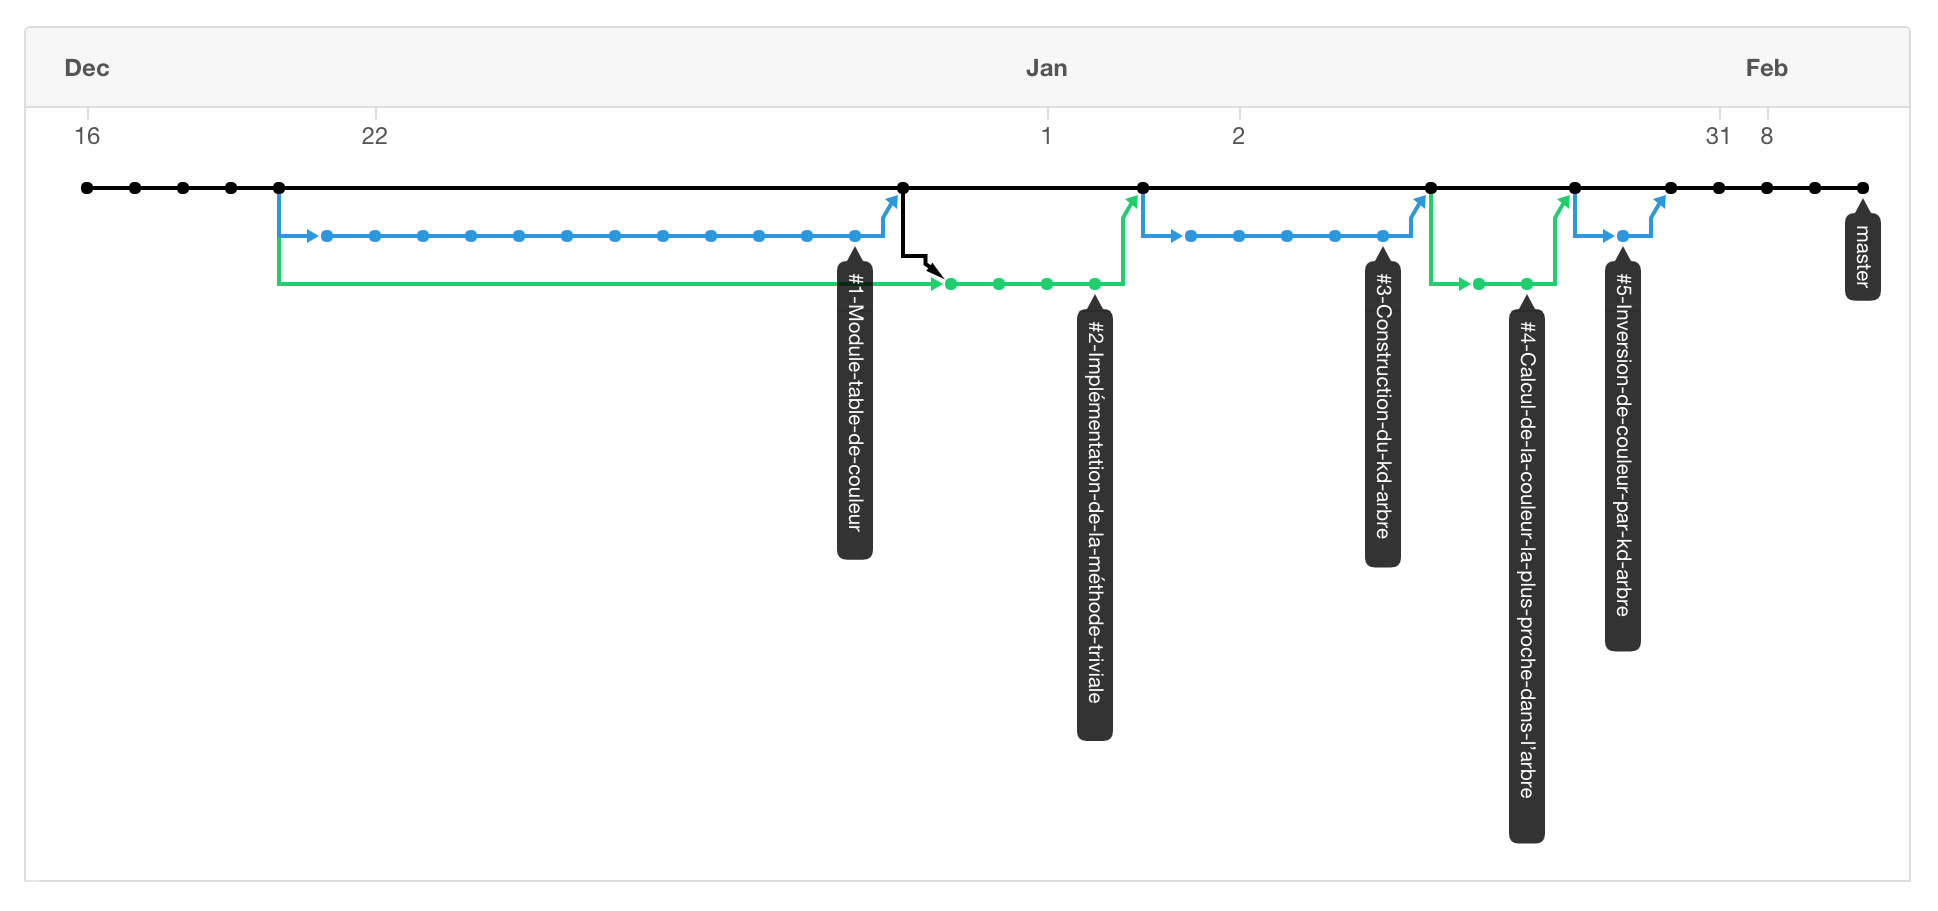
\includegraphics[width=150mm]{./pic/gitTree.jpg}
	\caption{Arbre des commits Git}
\end{figure}

L’intégralité des commits sont disponibles à l’adresse suivante: \url{https://github.com/vDurand/ProjetC-Inversion/commits/master}

\section{Architecture}

\begin{figure}[!ht]
    \centering
    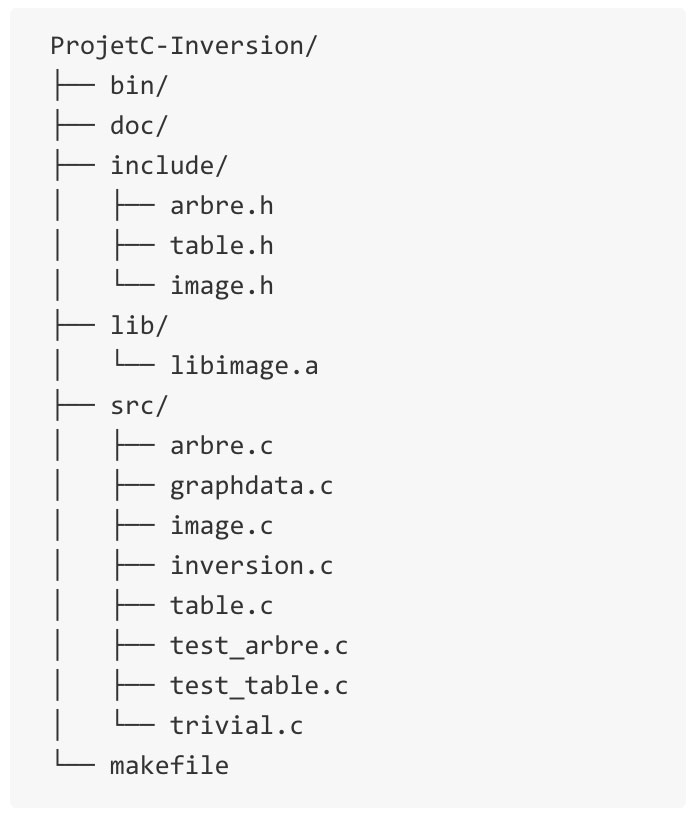
\includegraphics[width=70mm]{./pic/directoryStructure.jpg}
    \caption{Structure du répertoire projet}
\end{figure}

Afin de gérer les images \texttt{.ppm}, le programme exploite le module image sous forme du \texttt{image.c} compilé en librairie statique \texttt{libimage.a} contenu dans le dossier lib. Le makefile permet de compiler trois exécutables:
\begin{itemize}
\item \textbf{trivial} qui réalise l’inversion des couleurs par la méthode triviale ;
\item \textbf{inversion} qui réalise l’inversion des couleurs par le biais d’un kd arbre ;
\item \textbf{graphdata} qui permet de générer un fichier contenant les temps nécéssaires pour l’inversion une image par la méthode trivial et la méthode kd arbre avec des tables successivement de 128, 256, 512 et 1024 couleurs.
\end{itemize}

\section{Table de couleur}

\subsection{Structure des données}

Une table de couleur est une image de 1 pixel de hauteur sur le nombre de couleurs de la table. Pour stocker cette image, on utilise une structure \texttt{color\_table} qui contient un entier représentant le nombre de couleurs stockées, un booléen définissant si la table est une sous-table ou non (vrai si elle n’est pas une sous-table, faux sinon) et un pointeur de pointeur permettant d’allouer un tableau d’entiers à deux dimensions. Ce tableau a un nombre de colonnes égale au nombre de couleurs de la table et 3 lignes pour les composantes rouge, vert, bleu de chaque pixel. Cette représentation par tableau permet de trouver facilement une couleur par son index sans avoir à l’explorer.

\subsection{Fonctions}

\begin{itemize}
\item\texttt{create\_color\_table}: à partir d’une image on créé une table de couleur. Dans un premier temps on récupère le nombre de couleurs grâce à la fonction \texttt{image\_give\_largeur} du module image. On alloue ensuite les 3 lignes du tableau qui contiendront les composantes des couleurs, en fonction de la taille récupérée précédemment. Une fois ce tableau défini, on explore l’image pixel par pixel et on récupère leurs composantes RGB grâce à la fonction \texttt{image\_lire\_pixel} du module image, que l’on stocke dans le tableau d’entier ;
\item\texttt{destroy\_color\_table}: nettoie l’empreinte mémoire de la table de couleur. On libère l’espace mémoire de chaque ligne du tableau dans un premier temps, puis l’espace mémoire du reste de la structure. Attention on ne libère le tableau que si la table n’est pas une sous-table sinon la table mère serait corrompue ;
\item\texttt{color\_table\_duplicate}: crée une sous-table à partir d’une table mère. On alloue 3 pointeurs qui prendront l’adresse de la case du tableau de la table mère correspondant à la première case de la sous-table pour de chaque composante RGB. Ce qui équivaut à l’adresse de la première case du tableau de la table mère décalé du nombre de case où commence la nouvelle table fille ;
\item\texttt{color\_table\_get\_color}: retourne la couleur à une position précise dans la table sous la forme d’un tableau de taille 3 ;
\item\texttt{color\_table\_get\_nb\_color}: retourne ne nombre de couleurs présentes dans la table ;
\item\texttt{color\_table\_sort}: trie les couleurs suivant un axe RGB choisi ;
\item\texttt{color\_table\_get\_min} et \texttt{color\_table\_get\_max}: retourne la couleur la plus petite et la plus grande en fonction d’un axe RGB. Ces fonctions étaient utilisées pour la première version du choix de l’axe de coupe du kd arbre, mais sont devenues obsolètes avec la méthode de la variance.
\end{itemize}

\section{Méthode triviale}

On passe en argument le chemin d’une image et d’une table de couleur, on charge ensuite ces deux images grâce à la fonction image\_charger du module image. On crée la table de couleur à partir de la seconde image via la fonction \texttt{create\_color\_table}.
Puis l’inversion d’une image par une table de couleur se fait ici en comparant la distance entre la couleur de chaque pixel de l’image et toutes les couleurs de la table. On explore donc la table de couleur en entière autant de fois qu’il y a de pixel dans l’image. La distance est calculée en utilisant la formule:
\[
Distance = \sqrt{(c1[rouge]-c2[rouge])^2 + (c1[vert]-c2[vert])^2 + (c1[bleu]-c2[bleu])^2}
\]
On remplace ensuite la couleur de chaque pixel par la couleur de la table ayant la distance la plus faible avec celle-ci. L’image résultat est ensuite enregistrée grâce à la fonction \texttt{image\_sauvegarder} du module image.

\section{Kd arbre}

\subsection{Structure des données}

Un kd arbre est une suite de pointeur sur des noeuds liés entre eux. On utilise donc une structure \texttt{kdtree} qui représente un noeud et qui stocke 2 pointeurs vers son noeud fils droit et son noeud fils gauche. Si ce noeud est une feuille, ces 2 pointeurs sont nuls. Cette structure contient aussi une table de couleur. La racine de l’arbre contient la table complète avec toutes les couleurs puis son fils gauche contient la moitié trié inférieure à un plan de coupe de cette table et le fils droit la moitié supérieure. On coupe successivement la table à chaque noeuds jusqu’à ce que chaque feuille contiennent une infime portion de la table d’origine. Pour connaître le plan de coupe de chaque noeud, la structure comprend un pointeur vers une structure stockant les données du plan de coupe et un entier spécifiant l’axe de coupe RGB. Cette structure \texttt{cutting\_plane} possède un entier qui indique la position sur l’axe de coupe du noeud, de la couleur juste au dessus du plan de coupe dans la table et un entier contenant la valeur moyenne entre la composante de l’axe de coupe de la couleur juste au dessus du plan et celle juste en dessous.

\subsection{Fonctions}

\begin{itemize}
\item\texttt{choose\_sorting\_axis\_by\_max}: permet de sélectionner l’axe RGB de coupe en prenant celui qui a la plus grande différence entre sa composante de couleur maximum et sa composante de couleur minimum. Cette fonction est délaissé au profit de la méthode par la variance ;
\item\texttt{choose\_sorting\_axis\_by\_var}: permet de choisir l’axe RGB de coupe en fonction de celui qui a la plus grande variance. On calcule donc la moyenne de chaque composante RGB de toutes les couleurs de la table, puis on calcule la variance de chaque axe en faisant la somme des carrés de chaque composante moins la moyenne de cette composante, le tout divisé par le nombre de couleurs ;
\item\texttt{choose\_axis\_position}: retourne la position de la couleur juste au dessus du plan de coupe. On divise la table en deux et on vérifie bien que la valeur n’est pas la même des deux côtés du plan. Sinon on boucle jusqu’à ce que la valeur soit différence afin qu’on ait pas des couleurs à composantes identique sur un axe RGB de part et d’autre du plan de coupe ;
\item\texttt{create\_kdtree}: cette fonction permet de créer le kd arbre. Dans un premier temps on alloue l’espace mémoire pour le noeud racine, on lui associe la table de couleur au complet triée via la fonction \texttt{color\_table\_sort}, puis on définie l’axe et le plan de coupe grâce aux fonctions vues précédemment. Ensuite on définie récursivement les noeuds fils droit et gauche qui prennent respectivement la moitié supérieur et inférieur de la table de couleur du noeud père, et ce tant que le nombre de couleur au dessus ou en dessous du plan de coupe n’est pas inférieur au seuil prédéfini ;
\item\texttt{destroy\_kdtree}: supprime récursivement les fils des noeuds tant qu’ils ne sont pas nul, détruit la table de couleur et désalloue la structure \texttt{cuttingPlane} de chaque noeud ;
\item\texttt{get\_distance\_between\_colors}: calcul la distance entre deux couleurs avec la même formule que dans la méthode triviale ;
\item\texttt{search\_nearest\_color\_in\_node}: permet de trouver la couleur la plus proche dans la table spécifique d’un noeud à une couleur d’une image ;
\item\texttt{kdtree\_get\_nearest\_color}: cette fonction explore l’arbre pour trouver la feuille contenant la couleur la plus proche de la table de couleur à une couleur d’une image. La recherche se fait récursivement, si la couleur cherchée est sous le plan de coupe du noeud actuel on cherche à nouveau dans son fils gauche en rappelant \texttt{kdtree\_get\_nearest\_color} et si elle est au dessus du plan de coupe on cherche dans le fils droit. On descend ainsi dans l’arbre jusqu’à être dans la feuille qui pourrait contenir la couleur recherchée. On explore la partie de la table spécifique à cette feuille via la fonction \texttt{search\_nearest\_color\_in\_node} pour trouver la couleur la plus proche. Une fois cette couleur trouvé, on remonte l’arbre et on vérifie que la distance entre la couleur recherchée et la couleur trouvée est bien inférieure à la distance entre la couleur recherchée et la projetée de cette couleur sur le plan de coupe. Si ce n’est pas le cas, on est obligé de réeffectuer la recherche de la couleur la plus proche dans la table spécifique au noeud père, afin d’être sûr qu’il n’y a pas une couleur encore plus proche.
\end{itemize}

\section{Exécution}

\texttt{\$ ./inversion IMAGES/lenna.ppm IMAGES/TABLES/table\_house\_1280.ppm}

\begin{figure}[!ht]
    \centering
    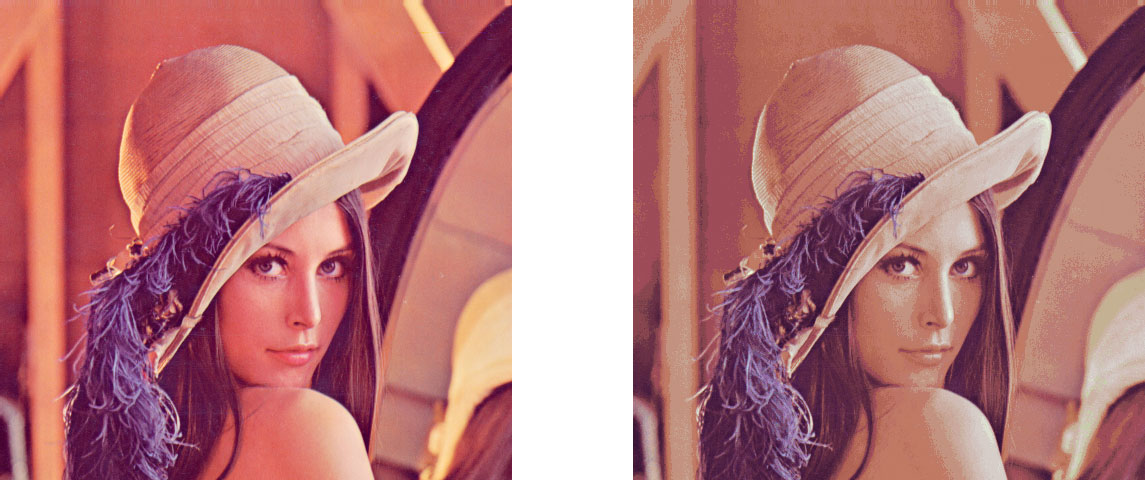
\includegraphics[width=150mm]{./pic/beforeAfter1280.jpg}
    \caption{Image Lenna avant/après inversion par table House 1280 couleurs et seuil 10}
\end{figure}

\cleardoublepage

\texttt{\$ ./inversion IMAGES/fleurs.ppm IMAGES/TABLES/table\_lenna\_53.ppm 5}

\begin{figure}[!ht]
    \centering
    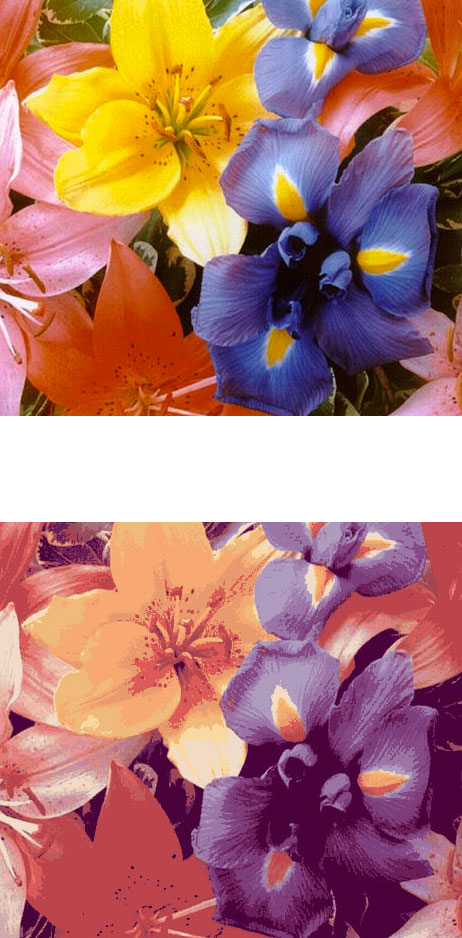
\includegraphics[width=90mm]{./pic/beforeAfter53v.jpg}
    \caption{Image Fleurs avant/après inversion par table Lenna 53 couleurs et seuil 5}
\end{figure}

\section{Conclusion}
\addcontentsline{toc}{section}{Conclusion}

La recherche par kd arbre assure un temps d’exécution nettement plus court pour les inversions par tables à grands nombres de couleurs. La différence ce note particulièrement lors de l’inversion par une table aux couleurs proches, comme par exemple l’inversion de l’image Lenna par la table Lenna générée à partir de cette même image, l’image n’est donc pas réellement inversée mais on a limité le nombre de couleurs utilisées. Les courbes de temps d'exécution ci-dessous ont été réalisés pour des tables de 128, 256, 512 et 1024 couleurs via \texttt{graphdata.c} et tracées par \texttt{gnuplot}.

\begin{figure}[!ht]
    \centering
    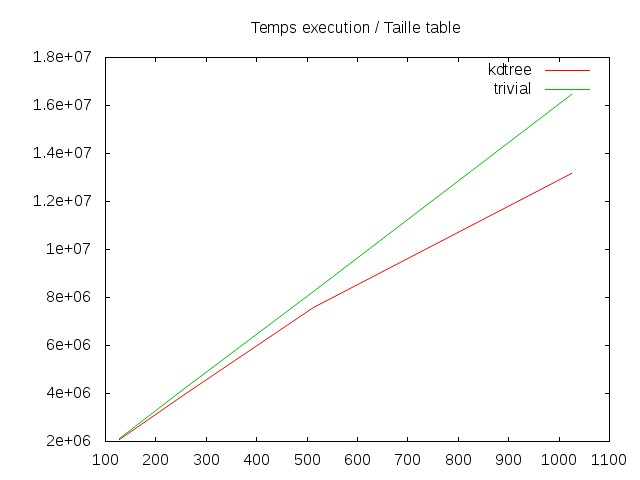
\includegraphics[width=90mm]{./pic/graphexec-dif.jpg}
    \caption{Image et table de couleur provenant de sources différentes}
\end{figure}

\begin{figure}[!ht]
    \centering
    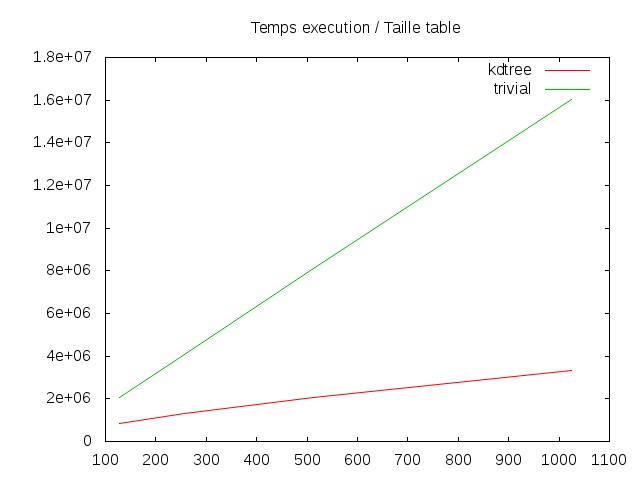
\includegraphics[width=90mm]{./pic/graphexec-meme.jpg}
    \caption{Image et table de couleur provenant de la même source}
\end{figure}

\end{document}